\documentclass[varwidth]{standalone}
\usepackage[utf8]{inputenc}
\usepackage{tikz}
\usetikzlibrary{%
    decorations.pathreplacing,%
    decorations.pathmorphing,%
    arrows,
    arrows.meta,
    positioning,
    shapes,
    shadows,
    shapes.geometric
    }

\definecolor{myblue1}{RGB}{0,157,209}
\definecolor{myblue2}{RGB}{161,224,255}
\definecolor{myblue3}{RGB}{216,229,245}
\definecolor{myblue4}{RGB}{0,149,229}

\tikzset{
  startend1/.style={
    rectangle, 
    rounded corners=15pt, 
    text width=2cm, 
    minimum height=1cm,
    align=center, 
    line width=2pt,
    draw=white,
    font=\color{white}\sffamily, 
    fill=myblue1,
    drop shadow
  },  
 data1/.style={
   trapezium, 
   trapezium left angle=70, 
   trapezium right angle=110, 
   text width=1.5cm, 
   inner ysep=17pt,
   align=center, 
   line width=2pt,
   draw=white,
   font=\color{black}\sffamily, 
   top color=myblue2,
   bottom color=myblue2!20,
   drop shadow
  },  
  process1/.style={
    rounded corners,
    text width=2.6cm, 
    minimum height=1.5cm, 
    align=center, 
    font=\color{white}\sffamily, 
    line width=2pt,
    draw=white, 
    top color=myblue1,
    bottom color=myblue1!30,
    drop shadow
  },  
  decision1/.style={
    diamond, 
    text width=1.5cm, 
    align=center, 
    font=\color{white}\sffamily, 
    line width=2pt,
    draw=white, 
    fill=myblue1,
    drop shadow
  },  
  arrow1/.style={
    {Square[]}->,
    myblue1,
    >=stealth
  },  
} 

\tikzset{
  startend2/.style={
    rectangle, 
    rounded corners=15pt, 
    text width=2cm, 
    minimum height=1cm,
    align=center, 
    line width=1pt,
   draw=myblue1!70!black, 
    font=\color{white}\sffamily, 
    fill=myblue1,
  },  
 data2/.style={
   trapezium, 
   trapezium left angle=70, 
   trapezium right angle=110, 
   text width=1.5cm, 
   inner ysep=17pt,
   align=center, 
   line width=1pt,
   draw=myblue1!70!black, 
   font=\color{black}\sffamily, 
   fill=myblue1,
  },  
  process2/.style={
    rounded corners,
    text width=2.6cm, 
    minimum height=1.5cm, 
    align=center, 
    font=\color{white}\sffamily, 
    draw=myblue1!70!black,
    line width=1pt, 
    fill=myblue1,
  },  
  decision2/.style={
    diamond, 
    text width=1.5cm, 
    align=center, 
    font=\color{white}\sffamily, 
    line width=1pt,
    draw=myblue1!70!black, 
    fill=myblue1,
  },  
  arrow2/.style={
     ->,
    myblue1,
    >=stealth
  },  
} 

\tikzset{
  startend3/.style={
    rectangle, 
    rounded corners=15pt, 
    text width=2cm, 
    minimum height=1cm,
    align=center, 
    line width=2pt,
    font=\color{myblue1}\sffamily, 
    fill=myblue3,
  },  
 data3/.style={
   trapezium, 
   trapezium left angle=70, 
   trapezium right angle=110, 
   text width=1.5cm, 
   inner ysep=17pt,
   align=center,
   draw=myblue1, 
   font=\color{myblue1}\sffamily, 
   fill=white
  },  
  process3/.style={
    text width=2.6cm, 
    minimum height=1.5cm, 
    align=center, 
    font=\color{white}\sffamily, 
    fill=myblue4,
  },  
  decision3/.style={
    diamond, 
    text width=1.5cm, 
    align=center, 
    font=\color{myblue1}\sffamily, 
    fill=myblue3,
  },  
  arrow3/.style={
    ->,
    myblue1,
    >=stealth
  },  
} 

\begin{document}

\begin{tikzpicture}[node distance=1.5cm and 2cm]
\node[startend1] 
  (start) 
  {start};
\node[decision1,below=of start] 
  (dec) 
  {dec1};
\node[process1,below=of dec] 
  (pro) 
  {process};
\node[data1,below=of pro] 
  (data) 
  {data};
\coordinate[below=of data] (aux);  
\node[startend1, below=of data] 
  (end) 

  {end};

\begin{scope}[arrow1]
\draw
  (start) --  (dec);
\draw
  (dec) --  node[fill=white] {yes} (pro);
\draw
  (dec) --  node[fill=white] {no} (data);
\draw
  (pro) |- (data);
\draw
  (data) |- (end);
\end{scope}  
\end{tikzpicture}

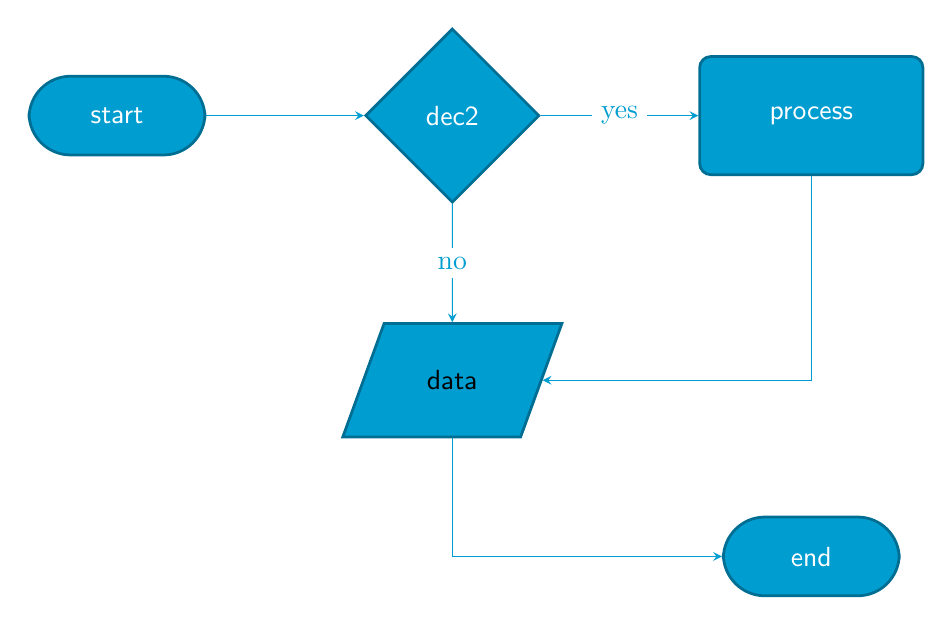
\begin{tikzpicture}[node distance=1.5cm and 2cm]
\node[startend2] 
  (start) 
  {start};
\node[decision2,right=of start] 
  (dec) 
  {dec2};
\node[process2,right=of dec] 
  (pro) 
  {process};
\node[data2,below=of dec] 
  (data) 
  {data};
\coordinate[below=of data] (aux);  
\node[startend2] 
  (end) 
  at (pro|-aux)
  {end};

\begin{scope}[arrow2]
\draw
  (start) --  (dec);
\draw
  (dec) --  node[fill=white] {yes} (pro);
\draw
  (dec) --  node[fill=white] {no} (data);
\draw
  (pro) |- (data);
\draw
  (data) |- (end);
\end{scope}  
\end{tikzpicture}

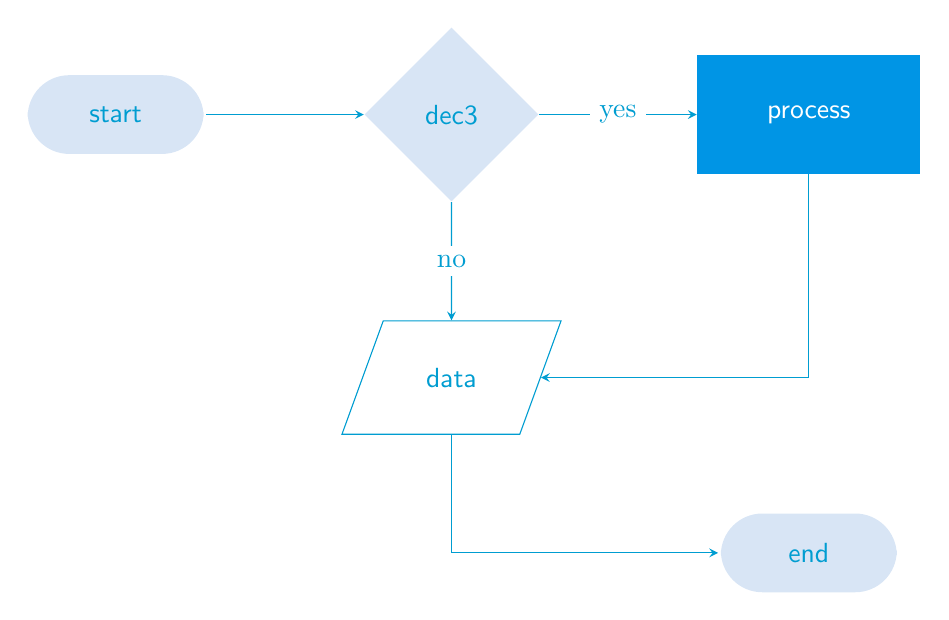
\begin{tikzpicture}[node distance=1.5cm and 2cm]
\node[startend3] 
  (start) 
  {start};
\node[decision3,right=of start] 
  (dec) 
  {dec3};
\node[process3,right=of dec] 
  (pro) 
  {process};
\node[data3,below=of dec] 
  (data) 
  {data};
\coordinate[below=of data] (aux);  
\node[startend3] 
  (end) 
  at (pro|-aux)
  {end};

\begin{scope}[arrow3]
\draw
  (start) --  (dec);
\draw
  (dec) --  node[fill=white] {yes} (pro);
\draw
  (dec) --  node[fill=white] {no} (data);
\draw
  (pro) |- (data);
\draw
  (data) |- (end);
\end{scope}  
\end{tikzpicture}

\end{document}
